\documentclass[xcolor=svgnames]{beamer}
\usetheme{Torino}

\usepackage{epsfig} %for figures
\usepackage{xcolor} %for color
\usepackage[utf8]{inputenc}
\usepackage{multicol}
\usepackage{hyperref}

% latex definitions:
\def\d{{\rm d}}
\def\half{{\textstyle{1\over2}}}



\title[SymPy\hspace{4em}\insertframenumber/
\inserttotalframenumber]{~\\ SymPy Tutorial \\~}


\author[O. Čertík, M. Paprocki, A. Meurer]
{Ondřej Čertík, Mateusz Paprocki, Aaron Meurer}

\pgfdeclareimage[height=1.5cm]{mylogo}{sympy-250px}
\institute{\pgfuseimage{mylogo}}

\date{June 24, 2013}

\begin{document}

\begin{frame}
  \maketitle
\end{frame}

\begin{frame}{Today's Tutorial}
\begin{center}
\Huge Welcome!
\end{center}

\normalsize All materials for today's tutorial are at \url{http://certik.github.io/scipy-2013-tutorial/}

\end{frame}

\begin{frame}{Outline}
  \begin{block}{SymPy Introduction}
    \begin{itemize}
    \item Goal
    \item Features
    \item History
    \item Present
    \item Future
    \end{itemize}
  \end{block}

  \begin{block}{Tutorial}
    \begin{itemize}
    \item Intro to SymPy and Basic features
    \item Solving real life problems
    \end{itemize}
  \end{block}
\end{frame}

\begin{frame}{SymPy Goal}
  \begin{block}{Goal}
    Provide a symbolic manipulation library in Python.
  \end{block}
  \pause
  \begin{block}

    ``SymPy is an open source Python library for symbolic mathematics. It aims to
    become a full-featured computer algebra system (CAS) while keeping the code as
    simple as possible in order to be comprehensible and easily extensible. SymPy
    is written entirely in Python and does not require any external libraries.''

  \end{block}
\end{frame}

\begin{frame}{Features}
  \begin{multicols}{2}
    \tiny
    \begin{itemize}
    \item \textbf{Core Capabilities}
      \begin{itemize}
        \tiny
      \item Basic arithmetic: Support for operators such as +, -, *, /, ** (power)
      \item Simplification
      \item Expansion
      \item Functions: trigonometric, hyperbolic, exponential, roots, logarithms,
        absolute value, spherical harmonics, factorials and gamma functions, zeta
        functions, polynomials, special functions, \ldots
      \item Substitution
      \item Numbers: arbitrary precision integers, rationals, and floats
      \item Noncommutative symbols
      \item Pattern matching
      \end{itemize}
    \item \textbf{Polynomials}
      \begin{itemize}
        \tiny
      \item Basic arithmetic: division, gcd, \ldots
      \item Factorization
      \item Square-free decomposition
      \item Gröbner bases
      \item Partial fraction decomposition
      \item Resultants
      \end{itemize}
    \item \textbf{Calculus}
      \begin{itemize}
        \tiny
      \item Limits: $\lim_{x\to 0}{x\log(x)} = 0$
      \item Differentiation
      \item Integration: It uses extended Risch-Norman heuristic
      \item Taylor (Laurent) series
      \end{itemize}
    \item \textbf{Solving equations}
      \begin{itemize}
        \tiny
      \item Polynomial equations
      \item Algebraic equations
      \item Differential equations
      \item Difference equations
      \item Systems of equations
      \end{itemize}
    \item \textbf{Combinatorics}
      \begin{itemize}
        \tiny
      \item Permutations
      \item Combinations
      \item Partitions
      \item Subsets
      \item Permutation Groups: Polyhedral, Rubik, Symmetric, \ldots
      \item Prufer and Gray Codes
      \end{itemize}

    \end{itemize}
  \end{multicols}
\end{frame}

\begin{frame}{Features}
  \begin{multicols}{2}
    \begin{itemize}
      \tiny
    \item \textbf{Discrete math}
      \begin{itemize}
        \tiny
      \item Binomial coefficients
      \item Summations
      \item Products
      \item Number theory: generating prime numbers, primality testing, integer
        factorization, \ldots
      \item Logic expressions
      \end{itemize}

    \item \textbf{Matrices}
      \begin{itemize}
        \tiny
      \item Basic arithmetic
      \item Eigenvalues/eigenvectors
      \item Determinants
      \item Inversion
      \item Solving
      \item Abstract expressions
      \end{itemize}


    \item \textbf{Geometric Algebra}


    \item \textbf{Geometry}
      \begin{itemize}
        \tiny
      \item points, lines, rays, segments, ellipses, circles, polygons, \ldots
      \item Intersection
      \item Tangency
      \item Similarity
      \end{itemize}

    \item \textbf{Plotting}
      \begin{itemize}
        \tiny
      \item Coordinate modes
      \item Plotting Geometric Entities
      \item 2D and 3D
      \item Interactive interface
      \item Colors
      \end{itemize}

    \item \textbf{Physics}
      \begin{itemize}
        \tiny
      \item Units
      \item Mechanics
      \item Quantum
      \item Gaussian Optics
      \item Pauli Algebra
      \end{itemize}

    \item \textbf{Statistics}
      \begin{itemize}
        \tiny
      \item Normal distributions
      \item Uniform distributions
      \item Probability
      \end{itemize}

    \item \textbf{Printing}
      \begin{itemize}
        \tiny
      \item Pretty printing: ASCII/Unicode pretty printing, LaTeX
      \item Code generation: C, Fortran, Python
      \end{itemize}
    \end{itemize}
  \end{multicols}
\end{frame}

\begin{frame}{History}
  \begin{block}{History}
    \begin{itemize}
    \item Ondřej Čertík started the project in 2006.
    \item Development took off in 2007 when SymPy first participated in Google
      Summer of Code. We have participated in every Google Summer of Code since.
    \item In 2011, Aaron Meurer (who also joined from Google Summer of Code) took
      over as lead developer.
    \end{itemize}
  \end{block}
\end{frame}

\begin{frame}{Present}
  \begin{block}{Current Status}
    \begin{itemize}
    \item Over 250 contributors.
    \item Current code base has over 400,000 lines of code and documentation.
    \item We have crossed the point of ``sympy a toy'' to ``sympy a tool''
    \end{itemize}
  \end{block}
\end{frame}

\begin{frame}{Future}
  \begin{block}{GSoC}
    These are our current GSoC projects. Expect to see these features by the end
    of the summer.
    \begin{itemize}
    \item \normalsize Risch algorithm for symbolic integration: \small Chetna Gupta
    \item \normalsize Faster Algorithms for Polynomials over Algebraic Number Fields: \small Katja Sophie Hotz
    \item \normalsize Improved ODE Solver in SymPy: \small Manoj Kumar
    \item \normalsize Lie Algebras: \small Mary Clark
    \item \normalsize Vector calculus module: \small Prasoon Shukla
    \item \normalsize Addition of electromagnetism features to sympy.physics: \small Sachin Joglekar
    \item \normalsize Diophantine Equation Module for SymPy: \small Thilina Rathnayake
    \end{itemize}
  \end{block}
\end{frame}

\begin{frame}{Future}
\begin{block}{Other Plans}
\begin{itemize}
\item New assumptions
\item Make things faster
\item Implement more algorithms, so we can compute more things (and also make
  them faster)
\item Make it easier for people to define custom behavior of their own objects
  in Add and Mul
\item Encourage people to use SymPy for many applications
\item https://github.com/sympy/sympy/wiki/gsoc-2013-ideas for full list of
  things we want done
\end{itemize}
\end{block}
\end{frame}

\begin{frame}{Git Commits Plots}
  \begin{block}{Last Year}
    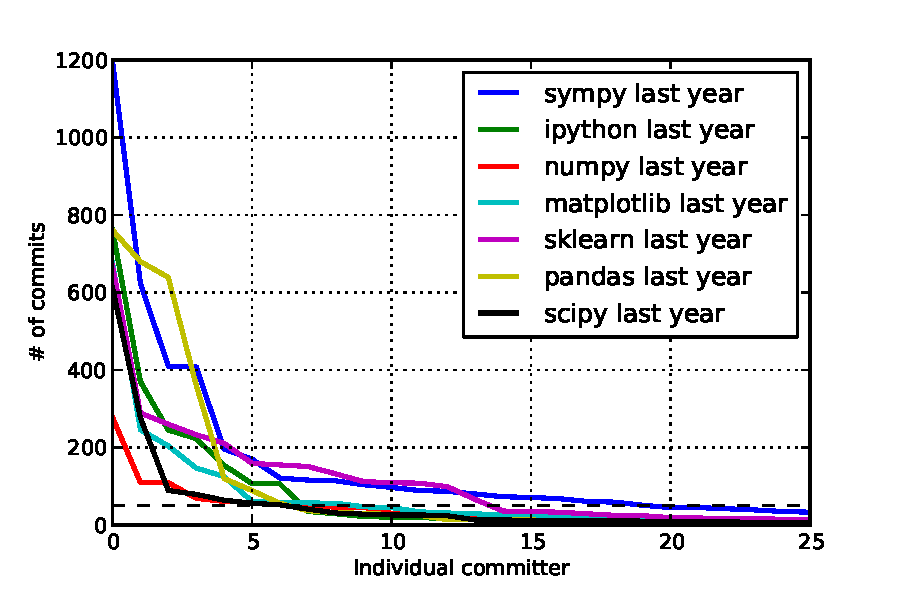
\includegraphics[width=4in]{commits1.pdf}
  \end{block}
\end{frame}

\begin{frame}{Git Commit Plots}
  \begin{block}{Last Year}
    \begin{itemize}
    \item The dotted line is 50 commits.
    \item Rough measurement of each project's ``bus factor''
    \end{itemize}
  \end{block}
\end{frame}

\begin{frame}{Git Commits Plots}
  \begin{block}{All Time}
    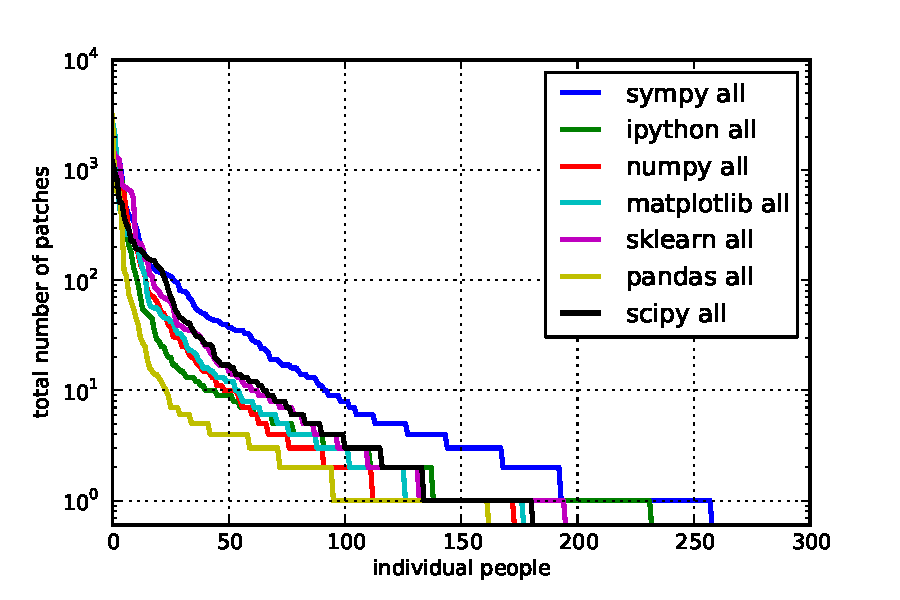
\includegraphics[width=4in]{commits-all.pdf}
  \end{block}
\end{frame}

\begin{frame}{Git Commit Plots}
  \begin{block}{All Time}
    \begin{itemize}
    \item SymPy has more total contributors\footnote{some of the other projects are actually exaggerated,
        because they don't use \texttt{.mailmap}}
    \item SymPy has a very welcome and friendly community, which is open, and
      actively encourages contributions.
    \item The SymPy code base is very approachable to new contributors.
    \item To be fair, Google Code-In accounts for a lot of this\ldots
    \end{itemize}
  \end{block}
\end{frame}

\begin{frame}{Authors}
  \begin{multicols}{5}
    \tiny
    Chris Smith\\
    Aaron Meurer\\
    Mateusz Paprocki\\
    Ondřej Čertík\\
    Matthew Rocklin\\
    Julien Rioux\\
    Ronan Lamy\\
    Raoul Bourquin\\
    Kirill Smelkov\\
    Øyvind Jensen\\
    Tom Bachmann\\
    Sergiu Ivanov\\
    Mario Pernici\\
    Saptarshi Mandal\\
    Stefan Krastanov\\
    Brian E. Granger\\
    Vinzent Steinberg\\
    Vladimir Perić\\
    Raymond Wong\\
    Sergey B Kirpichev\\
    David Li\\
    Fredrik Johansson\\
    Sean Vig\\
    Fabian Pedregosa\\
    Bharath M R\\
    Gilbert Gede\\
    Addison Cugini\\
    Thomas Hisch\\
    Guru Devanla\\
    Priit Laes\\
    Prasoon Shukla\\
    Alexey U. Gudchenko\\
    Matt Habel\\
    Tomo Lazovich\\
    Matt Curry\\
    Timothy Reluga\\
    Jason Gedge\\
    Aleksandar Makelov\\
    Sachin Joglekar\\
    Brian Jorgensen\\
    Kendhia\\
    Andy R. Terrel\\
    Ramana Venkata\\
    Grzegorz Świrski\\
    Sebastian Krämer\\
    Pearu Peterson\\
    Manoj Kumar\\
    Toon Verstraelen\\
    Siddhanathan Shanmugam\\
    Joan Creus\\
    Jorn Baayen\\
    Christian Muise\\
    Jeremias Yehdegho\\
    Joachim Durchholz\\
    Kevin Hunter\\
    Riccardo Gori\\
    Matthew Hoff\\
    Steve Anton\\
    hm\\
    Sanket Agarwal\\
    Robert Schwarz\\
    David Ju\\
    Luke Peterson\\
    Angadh Nanjangud\\
    Bilal Akhtar\\
    Stepan Roucka\\
    Miha Marolt\\
    Renato Coutinho\\
    Saurabh Jha\\
    Niklas Thörne\\
    Alexander Hirzel\\
    Nathan Alison\\
    jerryma1121\\
    Brian Stephanik\\
    Sam Sleight\\
    Sachin Irukula\\
    Robert Kern\\
    Patrick Lacasse\\
    Angus Griffith\\
    Swapnil Agarwal\\
    Gary Kerr\\
    Sherjil Ozair\\
    Natalia Nawara\\
    Nicolas Pourcelot\\
    Huijun Mai\\
    Jim Zhang\\
    Ljubiša Moćić\\
    Prafullkumar P. Tale\\
    Marek Šuppa\\
    Freddie Witherden\\
    Roberto Nobrega\\
    Jason Moore\\
    Felix Kaiser\\
    Sean Ge\\
    Alan Bromborsky\\
    Chetna Gupta\\
    Friedrich Hagedorn\\
    Saroj Adhikari\\
    CJ Carey\\
    Jaroslaw Tworek\\
    Alexey Subach\\
    Yuri Karadzhov\\
    Rishabh Dixit\\
    Christian Bühler\\
    Ryan Krauss\\
    Min Ragan-Kelley\\
    Demian Wassermann\\
    Christopher Dembia\\
    Sam Magura\\
    Ananya\\
    Mark Dewing\\
    Raphael Michel\\
    Andreas Kloeckner\\
    Tarun Gaba\\
    Christophe Saint-Jean\\
    Tobias Lenz\\
    Tomasz Buchert\\
    Davy Mao\\
    Ankit Agrawal\\
    Nichita Utiu\\
    Piotr Korgul\\
    Mary Clark\\
    Harold Erbin\\
    Matthew Brett\\
    Chris Wu\\
    Chancellor Arkantos\\
    Katja Sophie Hotz\\
    Alexandr Popov\\
    Abderrahim Kitouni\\
    Stefano Maggiolo\\
    Varun Joshi\\
    Thilina Rathnayake\\
  \end{multicols}
\end{frame}

\begin{frame}{Authors}
  \begin{multicols}{5}
    \tiny
    Nimish Telang\\
    Tiffany Zhu\\
    Khagesh Patel\\
    Rom le Clair\\
    Imran Ahmed Manzoor\\
    Jochen Voss\\
    Stefen Yin\\
    David Roberts\\
    Sebastian Kreft\\
    Óscar Nájera\\
    Tristan Hume\\
    Florian Mickler\\
    Pan Peng\\
    Akshay Srinivasan\\
    Akshit Agarwal\\
    Amit Jamadagni\\
    Andrew Straw\\
    Barry Wardell\\
    Benjamin McDonald\\
    Bill Flynn\\
    Case Van Horsen\\
    Cristóvão Sousa\\
    Emma Hogan\\
    Geoffry Song\\
    George Waksman\\
    Jens H. Nielsen\\
    Julio Idichekop Filho\\
    Luca Weihs\\
    Luis Garcia\\
    Manoj Babu K.\\
    Martin Povišer\\
    Nikolay Lazarov\\
    Oliver Lee\\
    Raffaele De Feo\\
    Shravas K Rao\\
    Ted Horst\\
    Oscar Benjamin\\
    Michael Mayorov\\
    David Marek\\
    Goutham Lakshminarayan\\
    Ben Goodrich\\
    Jezreel Ng\\
    Tomáš Bambas\\
    Ashwini Oruganti\\
    Arpit Goyal\\
    Stephen Loo\\
    Jurjen N.E. Bos\\
    Colleen Lee\\
    James Aspnes\\
    Sai Nikhil\\
    Jack McCaffery\\
    Fernando Perez\\
    Oleksandr Gituliar\\
    Thomas Dixon\\
    Bradley Froehle\\
    Nikhil Sarda\\
    tsmars15\\
    Thomas Wiecki\\
    Pavel Fedotov\\
    Boris Timokhin\\
    Henrik Johansson\\
    James Abbatiello\\
    Sebastian Krause\\
    Hubert Tsang\\
    Gregory Ksionda\\
    Seshagiri Prabhu\\
    Shai 'Deshe' Wyborski\\
    Gert-Ludwig Ingold\\
    Acebulf\\
    Shruti Mangipudi\\
    Siddhant Jain\\
    Srinivas Vasudevan\\
    Elrond der Elbenfuerst\\
    Eh Tan\\
    David Lawrence\\
    Stepan Simsa\\
    Comer Duncan\\
    Takafumi Arakaki\\
    Tarang\\
    Christian Schubert\\
    Łukasz Pankowski\\
    Carsten Knoll\\
    Thomas Sidoti\\
    Tim Lahey\\
    Björn Dahlgren\\
    Bernhard R. Link\\
    Benjamin Fishbein\\
    Bastian Weber\\
    Tyler Pirtle\\
    Andrew Docherty\\
    Vasily Povalyaev\\
    Vinay Kumar\\
    Or Dvory\\
    Vladimir Lagunov\\
    Andre de Fortier Smit\\
    Anatolii Koval\\
    Ali Raza Syed\\
    Alexandr Gudulin\\
    marshall2389\\
    vishal\\
    Pauli Virtanen\\
    Andrej Tokarčík\\
    Prateek Papriwal\\
    Puneeth Chaganti\\
    Alexander Eberspächer\\
    Randy Heydon\\
    Nicholas J.S. Kinar\\
    Max Hutchinson\\
    Matthias Toews\\
    Matthew Tadd\\
    Matt Rajca\\
    Rizgar Mella\\
    Robert\\
    Robert Cimrman\\
    Marcin Kostrzewa\\
    Madeleine Ball\\
    Roberto Colistete, Jr.\\
    Konrad Meyer\\
    Kibeom Kim\\
    Kevin Goodsell\\
    Kazuo Thow\\
    Kaifeng Zhu\\
    Joseph Dougherty\\
    Jorge E. Cardona\\
    Johann Cohen-Tanugi\\
    James Pearson\\
  \end{multicols}
\end{frame}

\begin{frame}{Here at SciPy}
  \begin{block}{Talks}
    \begin{itemize}
    \item Matthew Rocklin, \textit{Matrix Expressions and BLAS/LAPACK}. \\ \footnotesize Thursday 10:15
      AM - 10:35 AM General - Rm 204
    \item \normalsize Jason Moore, \textit{Dynamics with SymPy Mechanics}. \\ \footnotesize 02:10 PM - 02:30
      PM General - Rm 204
    \item \normalsize David Li, \textit{SymPy Gamma and SymPy Live: Python and Mathematics
        Online}. \\ \footnotesize 03:50 PM -
      04:10 PM General - Rm 203 (High School student!)
    \end{itemize}
  \end{block}
  \begin{block}{Sprints}
    Come sprint with us!
    \begin{itemize}
    \item Releasing SymPy 0.7.2
    \item Lot's of tasks that are easy for new contributors
    \item Friday and Saturday
    \end{itemize}
  \end{block}
\end{frame}

\begin{frame}
\Huge Let's begin!
\end{frame}
\end{document}
